\documentclass[12pt,letterpaper]{article}
\usepackage[utf8]{inputenc}
\usepackage[document]{ragged2e}
\usepackage{enumitem}
\usepackage{blindtext}
\usepackage{amsmath, amsthm, amssymb}
\newtheorem{mydef}{Definition}
\newtheorem{prop}{Proposition}
\usepackage{tikz}
\newcommand*{\plogo}{\fbox{$\mathcal{PL}$}} 
\usepackage[T1]{fontenc}
\usepackage{stix}
\usepackage{titlesec}
\graphicspath{ {./pic/} }
\usetikzlibrary{arrows}
\usetikzlibrary{calc}
\usepackage{lastpage}
\usepackage{biblatex} %Imports biblatex package
\addbibresource{sample.bib} %Import the bibliography file
\usepackage{amssymb}
\usepackage{geometry}
\geometry{letterpaper, portrait, margin=2.5cm}
\linespread{2.0}
%%%%%%%%%%%%%%%%%%%%%%%%%%%%%%%%%%%%%%%%%%%%%%%%%%%%%%%%%%%%%%%%%%%%%%%%%%%%%%%%%%%%%%%%%%%%%%%%%%%%%%%%%%%%%%%%%%
\begin{document}
\begin{normalsize}
\begin{titlepage}

	\raggedleft 
	\rule{1pt}{\textheight}
	\hspace{0.05\textwidth} 
	\parbox[b]{0.75\textwidth}{ 
		{\Huge\bfseries Honours Research \\ Topology}\\[2\baselineskip]
		 
		{\Large\textsc{Ziang Wang}}  \\[10pt]
            {\Large{April 18, 2023}} 
		\vspace{0.5\textheight}
  
		{\noindent Marianoplis College~~}\\[\baselineskip]
	}
\end{titlepage}
\newpage
\tableofcontents
\newpage
%%%%%%%%%%%%%%%%%%%%%%%%%%%%%%%%%%%%%%%%%%%%%%%%%%%%%%%%%%%%%%%%%%%%%%%%%%%%%%%%%%%%%%%%%%%%%%%%%%%%%%%%%%%%%%%%%%
\section{Introduction}
\hspace{5mm} Topology, a branch in Math that extends into almost every theory, underlies the foundation for some of the most important theorems existed. Starting with topological space, it creates a group that is under the operation of subspace. Then by using homology and quotient vector space, we can solve geometric problem using algebra. Some applications include Betti Numbers and homotopic. Each Betti number of different dimensions represents a unique character of the object. A python code is enclosed at the end of this paper to  analyze the Betti number of any given data. Homotopy compares between data sets on whether or not they have similar structures and shapes. To start with, I will introduce some general topology definitions, and then cubical topology and homology following with a dimensional theorem.
%%%%%%%%%%%%%%%%%%%%%%%%%%%%%%%%%%%%%%%%%%%%%%%%%%%%%%%%%%%%%%%%%%%%%%%%%%%%%%%%%%%%%%%%%%%%%%%%%%%%%%%%%%%%%%%%%%
\section{Topology}
\hspace{5mm} We will start with general topology. In this section, I will first introduce some formal definitions that are necessary for defining boundary. 
\subsection{Norm Function}     
\begin{mydef}\label{def:def444}  
A function is called a norm if it has the following properties: 
$$||x|| = 0 \Longleftrightarrow x=0 \quad\textrm{for}\quad  \forall x \in \mathbf{R}^d$$
$$||cx|| = |c| \cdot ||x|| \quad\textrm{for}\quad \forall x \in \mathbf{R}^d \textbf{ and } \forall c \in \mathbf{R}$$
$$||x+y|| \leqslant ||x|| + ||y|| \quad \textrm{for}\quad \forall x,y \in \mathbf{R}^d$$
\end{mydef}
Norm is obviously only applicable in metric space. The followings are the most common forms of norm function. \\
\textbf{Dist function:}
$$X \times Y \longrightarrow \mathbf{R}^+$$
$$dist(x,y) \longrightarrow \mathbf{R}^+$$
\begin{enumerate}
    \item $dist_0(x,y)=||x-y||_0=max\{|x_1-y_1|, \textbf{ ... } ,|x_d-y_d|\}$
    \item $dist_1(x,y)=||x-y||_1=\sum_{i=1}^{d}|x_i-y_i|$
    \item $dist_2(x,y)=||x-y||_2=\sqrt{(x_1-y_1)^2+ \textbf{ ... }+(x_n-y_n)^2}$
\end{enumerate}
The most common one is obviously $dist_2(x,y)$.
%%%%%%%%%%%%%%%%%%%%%%%%%%%%%%%%%%%%%%%%%%%%%%%%%%%%%%%%%%%%%%%%%%%%%%%%%%%%%%%%%%%%%%%%%%%%%%%%%%%%%%%%%%%%%%%%%%
\subsection{Closed and Open set}
Now we introduce what is an open set.
\begin{mydef}\label{def:def444}  
A set $V\subset X$ is open iff for every point $x \in V$, there exists an $\epsilon > 0$ such that $B(x,y) \in V$.
\end{mydef}
Where$$B(x,y) = \{y \in X\textbf{ } | \textbf{ }dist(x,y) <r\}$$ \\
And a closed set is defined as,
\begin{center}
    If $x$ is open in $X$, then $X \setminus x$ is closed.
\end{center}
Noted, $B(x,y)$ is sometimes refers to as an epsilon ball. A way of understand this is by thinking open set contains every point in each epsilon ball around its boundary but not the boundary. Also, how the space $X$ is defined influences whether a set is open or not. $\mathbf{Z}$ is obviously not open in $\mathbf{R}$ but it is open if the space is itself.

\subsection{Closure}
\begin{mydef}\label{def:def444} 
The closure of A in X is defined as: 
$$cl(A)= \bigcap \{K_a\}$$
where $\{K_a\}$ is the collection of all the closed sets in $X$ containing $A$.
\end{mydef}
\subsection{Boundary Operator}
Some readers might already foresee how boundary operator would be defined. 
$$bd_xA=cl(A) \bigcap cl(X \setminus A)$$

%%%%%%%%%%%%%%%%%%%%%%%%%%%%%%%%%%%%%%%%%%%%%%%%%%%%%%%%%%%%%%%%%%%%%%%%%%%%%%%%%%%%%%%%%%%%%%%%%%%%%%%%%%%%%%%%%%
\section{Cubical Topology} 
\hspace{5mm} Cubical topology provides us an intuitive way of thinking graphs. It is very computational thanks to its rigid form.  \\
\subsection{Elementary Cube}
\hspace{5mm} In order to define elementary cube, we first define what is an elementary interval. \\ 

\begin{mydef}\label{def:def444} 
Elementary interval: 
        If $l \in \mathbb{R}$, a closed interval in $\mathbb{R}$ that has the form of \texttt{I} $ = [ l,l+1 ]$ or $[ l ]$ is called elementary interval.
  

\end{mydef}
\begin{itemize}
        \item  $[ l,l+1 ]$ is called non degenerated component 
        \item  $[ l ]$ is called degenerated component 
    \end{itemize}

\begin{mydef}\label{def:def444} 
 Elementary Cube: \\
        If Q is a finite product of elementary intervals, namely, \\
                     \begin{center}
                          $Q =$ \texttt{I_1}$\times$\texttt{I_2} $\times$\texttt{I_3} $...$ $\times$\texttt{I_d}, \\
                     \end{center} 
        \textsf{Q is then an elementary cube.}
\end{mydef}

\begin{itemize}
        \item $d$ is called the embedding number. $emb(Q) = d$
        \item The dimension of Q is the number of non degenerated components in Q.
        \item $K^d_n$ means the collection that contains every elementary cubes in a space that has the dimension n and embedding number d.
    \end{itemize}
\subsection{Cubical Chain}
After defining elementary cube, we will go further in the abstract world by defining a space. Imagine each elementary cube as an independent unit vector, the space that it generates can be expressed by something called k-chain.
\begin{mydef}\label{def:def444} 
K-chain:  \\
        K-chain is the span of numerous elementary cubes. \\
        Or, 
        let $\alpha_1, \alpha_2 ...$ be every $\mathbb{R}$, k-chain for $Q_1, Q_2 ...$ is \\
        $$C = \sum \alpha_i \cdot \widehat{Q_i}$$
        
\end{mydef}
\subsection{Cubical Product}
After having a space, we can perform operation in this space. The first that comes in mind is multiple. Multiplication in daily life is limited in $\mathbf{R}\times \mathbf{R}$, however we can extend this limit by using cubical product.
\begin{mydef}\label{def:def444}  
The cubical product of two elementary cubes is defined as
$$\widehat{P} \diamond \widehat{Q} = \widehat{P \times Q}$$
\\[10pt]
\end{mydef}

\begin{mydef}\label{def:def444} 
Let $c_1 \in K_K$ and $c_2 \in K'_K$. Cubical product is defined as
$$c_1 \diamond c_2 = \sum_{p\in K_K,Q \in K'_K}<c_1, \widehat{P}><c_2, \widehat{Q}> \widehat{P \times Q}$$
\\[10pt]
\end{mydef}

\begin{mydef}\label{def:def444} 
Let $c_1=\sum \alpha_i \cdot \widehat{Q_i}$ and $c_2=\sum \beta_i \cdot \widehat{Q_i}$. Scalar product of two k-chains is defined as
$$<c_1,c_2>=\sum_{i=1}^m\alpha_i \beta_i$$
\end{mydef}

\begin{mydef}\label{def:def444} 
Support of a chain is defined as
$$|c|=\bigcup \{ Q \in K_K^d\mbox{ } | \mbox{ }c(Q) \neq 0\}$$
\end{mydef} 

These are some interesting properties of cubical product. 
\begin{prop}
$$c_1 \diamond 0 = 0 \diamond c_1 = 0$$ 
\\[20pt]
\newpage
\textbf{Proof:} \\
Let $c_1=\sum a_i \widehat{Q_i}$. And $1 \le i,j \le emb(c_1)$. We can consider 0 as a k-chain with all its coefficients as 0, we name it $c_2=\sum 0 \cdot \widehat{Q_i}$. Therefore, $<c_2,\widehat{Q_j}>= 0 \cdot \widehat{Q_j}=0$, for $\forall Q_i \in K_K$, so $c_1 \diamond 0=c_1 \diamond c_2= \sum <c_1, \widehat{Q_i}> \cdot 0 \cdot \widehat{Q_i \times Q_j}=0$. And also since $ \sum <c_1, \widehat{Q_i}> \cdot 0 \cdot \widehat{Q_i \times Q_j}=  \sum 0 \cdot <c_1, \widehat{Q_i}>  \cdot \widehat{Q_j \times Q_i}$, $c_1 \diamond 0= 0 \diamond c_1$. Proven.
\\[20pt]
\end{prop}

\begin{prop}
$$c_1 \diamond (c_2 +c_3) = c_1 \diamond c_2 + c_1 \diamond c_3$$
 where $c_2,c_3 \in C_K^d$ \\[10pt]
\textbf{Proof:} \\
Let $c_1=\sum a_i \widehat{P_i}$, $c_2=\sum b_j \widehat{Q_j}$, $c_3=\sum c_j \widehat{Q_j}$. And $1 \le i \le emb(c_1)$, $1 \le j \le emb(c_2)$. We assign $c_2,c_3$ with the same elementary cubes $Q_j$ due to the fact that they are in the same $C_K^d$. Therefore, $c_1 \diamond (c_2 + c_3)=c_1 \diamond (\sum_{j}(b_j+c_j)\widehat{Q_j})=\sum_{i,j} a_i \cdot 1 \cdot (b_j+c_j) \cdot 1 \cdot \widehat{P_i \times Q_j}= \sum a_i  \cdot b_j \cdot \widehat{P_i \times Q_j} +\sum a_i  \cdot c_j \cdot \widehat{P_i \times Q_j}=c_1 \diamond c_2 + c_1 \diamond c_3$. Proven.
\\[20pt]
\end{prop}

\begin{prop}
$$(c_1 \diamond c_2) \diamond c_3 = c_1 \diamond (c_2 \diamond c_3)$$ 
\textbf{Proof:} \\
Let $c_1=\sum a_i \widehat{P_i}$, $c_2=\sum b_j \widehat{Q_j}$, $c_3=\sum c_k \widehat{W_k}$. And $1 \le i \le emb(c_1)$, $1 \le j \le emb(c_2)$, $1 \le j \le emb(c_3)$. Therefore, $(c_1 \diamond c_2) \diamond c_3 = (\sum_{i,j} a_i \cdot b_j \cdot \widehat{P_i \times Q_j}) \diamond c_3$ which is in the form of k-chain. We can consider the product as a chain with the coefficient of $a_i \cdot b_j$ and elementary cube as $\widehat{P_i \times Q_j}$. Thus,  $(\sum_{i,j} a_i \cdot b_j \cdot \widehat{P_i \times Q_j}) \diamond c_3=\sum_{i,j,k} a_i \cdot b_j \cdot c_k \cdot \widehat{P_i \times Q_j \times W_k} $. If we consider a chain with the coefficient of $b_j \cdot c_k$ and elementary cube as $\widehat{Q_j \times W_k}$, $\sum_{i,j,k} a_i \cdot b_j \cdot c_k \cdot \widehat{P_i \times Q_j \times W_k}= c_1 \diamond (\sum_{j,k} b_j \cdot c_k \cdot \widehat{Q_j \times W_k})=c_1 \diamond (c_2 \diamond c_3)$. Proven.
\\[20pt]
\end{prop}

\begin{prop}
$$\mbox{if } c_1 \diamond c_2=0 \mbox{, then } c_1=0 \mbox{ or } c_2=0$$ 
\textbf{Proof:} \\
Let $c_1=\sum a_i \widehat{P_i}$, $c_2=\sum b_j \widehat{Q_j}$. And $1 \le i \le emb(c_1)$, $1 \le j \le emb(c_2)$. So if $c_1 \diamond c_2=0$, then $\sum_{i,j}a_i \cdot b_j \cdot \widehat{P_i \times Q_j}=0$, for $\forall i,j$. In the case of either  $\widehat{Q}$ or  $\widehat{P}$ is all zero, the desired relation is obviously proven. When $\widehat{Q},\widehat{P} \neq 0$, $\sum_{i,j} a_i \cdot b_j=\sum a_i \cdot \sum b_j=0$. Therefore, either $\sum a_i=0 \mbox{ or } \sum b_i=0$. And if all the coefficients of a chain is 0, the the chain is obvious equal to 0. Proven.\\[20pt]
\end{prop}

\begin{prop}
$$|c_1 \diamond c_2|=|c_1| \times |c_2|$$ 
\textbf{Proof:} \\
Let $c_1=\sum a_i \widehat{P_i}$, $c_2=\sum b_j \widehat{Q_j}$. And $1 \le i \le emb(c_1)$, $1 \le j \le emb(c_2)$. So $|c_1 \diamond c_2|=|\sum a_i \cdot b_j \cdot \widehat{P_i \times Q_j}|=\{a_i \cdot b_j \cdot \widehat{P_i \times Q_j} \mbox{ } | \mbox{ }a_i \cdot b_j \neq 0\}$. And on the other side, $|c_1| \times |c_2|= \{a_i \cdot Q_i  \mbox{ } | \mbox{ }a_i \neq 0 \} \times \{b_j \cdot P_j  \mbox{ } | \mbox{ } b_j \neq 0 \}=\{a_i \cdot b_j \cdot \widehat{P_i \times Q_j} \mbox{ } | \mbox{ }a_i \neq 0 \mbox{, } b_j \neq 0\}$. And this set is equivalent to the previous set from the left hand side. Proven.
\end{prop}
\subsection{Boundary Operator}
\hspace{5mm} Now, for boundary. To find boundary generally, we want an operator($\partial_s$) that input a Q with dimension $s$ and return a Q' that has dimension $s-1$.\\
Some facts we know are: 
\begin{itemize}
    \item How $\partial_1$ works
            \begin{align*}
        \partial_1\colon  [l,l+1] &\mapsto [l+1] - [l]\\
                         [l] &\mapsto 0 
            \end{align*}
    \item For Q that $dim(Q)>1$, its each non degenerated interval will undergo $\partial_1$, degenerated interval will simply disappear. 
    \item The operator needs to have an order.
\end{itemize}
Without further due, this is the boundary operator for cubical set, it can be expressed in two ways. \\
Recursively defined,
    $$\partial_k \colon K^d_k \longrightarrow K^d_{k-1}$$
For $d>1$ let $I = I_1(Q)$, $P= I_2(Q) \times ... \times I_d(Q)$
$$\partial_k \widehat{Q}\textbf{ } =\textbf{ } \partial_k_1 \textbf{ } \widehat{I} \diamond \widehat{P} + (-1)^{k_1} \textbf{ }\widehat{I} \diamond \partial_k_2 \widehat{P}$$
where $k_1 = dim(I)$, $k_2=dim(P)$ \\[10pt]
Absolutely defined, \\
let $\{U_1,U_2 ...\}$ be the non degenerated interval, it is mixed with many degenerated ones\\
$$\partial \widehat{Q}\textbf{ } =\textbf{ } \sum \pm \partial \widehat{U_i} \diamond \{\widehat{Q_U_i}\} $$
where $\widehat{Q_U_i}$ is the interval list after $\widehat{U_i}$
%%%%%%%%%%%%%%%%%%%%%%%%%%%%%%%%%%%%%%%%%%%%%%%%%%%%%%%%%%%%%%%%%%%%%%%%%%%%%%%%%%%%%%%%%%%%%%%%%%%%%%%%%%%%%%%%%%
\newpage
\section{Homology}
\hspace{5mm} After defining boundary, we can define homology. Homology studies the connectivity properties of a giving graph. By using quotient, one can treat the boundary as the identity element to simplify the original group. In this section, we will introduce two ways of defining homology: in group and in vector space. 

\subsection{Path Function}
We will first define path function. 
\begin{mydef}\label{def:def444} 
 $$f: \quad [0,1] \mapsto X$$
\end{mydef}
This mapping is useful to show that every path can be represented by a function. In figure 1, one can see this mapping visually.
\usetikzlibrary {arrows.meta}
\begin{figure}[hbt!]
   
\begin{center}
    

\begin{tikzpicture}[scale=0.70]

\draw[-latex] (-0.8,1.5) -- (1.8,1.5) ; %edit here for the axis
\foreach \x in  {0,1} % edit here for the vertical lines
\draw[shift={(\x,1.5)},color=black] (0pt,3pt) -- (0pt,-3pt);
\foreach \x in {0,1} % edit here for the numbers
\draw[shift={(\x,1.5)},color=black] (0pt,0pt) -- (0pt,-3pt) node[below] 
{$\x$};
\draw[*-*] (-0.1,1.5) -- (1.1,1.5);
\draw[very thick] (-0.1,1.5) -- (1.1,1.5);

\draw[->] (3,1.5) -- (4,1.5);

% First, define nodes
\draw (6,0) node[circle, inner sep=0.8pt, fill=black, label={below:{$X_0$}}] (E) {};  
\draw (9,3) node[circle, inner sep=0.8pt, fill=black, label={below:{$X_1$}}] (F) {}; 

% Draw the curved line. No to[bend] is allowed, only explicit control points
\draw  (E) .. controls +(7.9,1) and +(4.1,1).. (F);
% Now, repeat the same curve, shifted up, and define 20 inner points named
% p1, p2, p3, etc.. for positions 0.15, 0.16, 0.17, etc up to 0.35 inside that curve
\path  ($(E)+(0,0.2)$) .. controls +(7.9,1) and +(4.1,1) ..  ($(F)+(0, 0.2)$)
 {\foreach \t [count=\i] in {0.15,0.16,...,0.35} {  coordinate[pos=\t] (p\i) } };

% Finally draw the "curve" (polygonal line indeed) through those 20 inner points
\draw[->>] (p1) { \foreach \i in {1,...,20} {-- (p\i) } };

\end{tikzpicture}
\caption{Path function}
    \label{fig:my_label}
\end{center}
\end{figure}

\subsection{Homotopy}
We can define homotopy now. Homotopy is an equivalent relation between two path functions. We can use this relation to generalize path functions. 
\begin{mydef}\label{def:def444} 
  $f$ and $f'$ are two continuous maps. If there is a continuous function $H$ that 
        $$H: \quad X \times [0,1] \rightarrow Y$$
        $$H(x,0)=f(x) \quad \textbf{and} \quad H(x,1)=f'(x)$$
        $f$ is then homotopic to $f'$, denoted as $f \simeq f'$
\end{mydef}
One can think of function $H$ as an animation from function $f_0$ to $f_1$. One interesting fact here: function $H$ has a domain in $\mathbf{R}^2$, more specifically $[0,1] \times [0,1]$.\\[10pt]
\begin{figure}[hbt!]
    \centering
    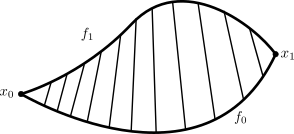
\includegraphics[scale=0.6]{1}
    \caption{Straight line homotopy}
    \label{fig:my_label}
\end{figure}
Figure 2 shows a straight line homotopy which is the easiest form of homotopy. \\
Homotopy equivalence relation generates an equivalent class. Equivalent class is a set that every two elements in this set are equivalent. Figure 3 shows three different path functions. All of them belong in the same equivalent class.
\begin{figure}[hbt!]
    \centering
   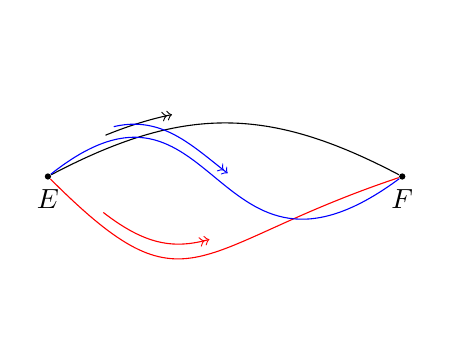
\begin{tikzpicture}[scale=0.9]

% First, define nodes
\draw (0,0) node[circle, inner sep=0.8pt, fill=black, label={below:{$E$}}] (E) {};  
\draw (5,0) node[circle, inner sep=0.8pt, fill=black, label={below:{$F$}}] (F) {}; 

% Draw the curved line. No to[bend] is allowed, only explicit control points
\draw  (E) .. controls +(1.9,1) and +(-1.9,1).. (F);
% Now, repeat the same curve, shifted up, and define 20 inner points named
% p1, p2, p3, etc.. for positions 0.15, 0.16, 0.17, etc up to 0.35 inside that curve
\path  ($(E)+(0,0.2)$) .. controls +(1.9,1) and +(-1.9,1) ..  ($(F)+(0, 0.2)$)
 {\foreach \t [count=\i] in {0.15,0.16,...,0.35} {  coordinate[pos=\t] (p\i) } };

% Finally draw the "curve" (polygonal line indeed) through those 20 inner points
\draw[->>] (p1) { \foreach \i in {1,...,20} {-- (p\i) } };

% A second example, with the same ideas but different path
\draw[red]  (E) .. controls +(2,-2) and +(-3,-1).. (F);
\path  ($(E)+(0,0.2)$) .. controls +(2,-2) and +(-3,-1)..  ($(F)+(0, 0.2)$) 
{\foreach \t [count=\i] in {0.15,0.16,...,0.55} {  coordinate[pos=\t] (p\i) } };

\draw[red, ->>] (p1) { \foreach \i in {1,...,40} {-- (p\i) } };

%third
\draw[blue]  (E) .. controls +(2.4,1.9) and +(-2.7,-2).. (F);
\path  ($(E)+(0,0.2)$) .. controls +(2.4,1.9) and +(-2.7,-2)..  ($(F)+(0, 0.2)$) 
{\foreach \t [count=\i] in {0.15,0.16,...,0.55} {  coordinate[pos=\t] (p\i) } };

\draw[blue, ->>] (p1) { \foreach \i in {1,...,40} {-- (p\i) } };

\end{tikzpicture}
    \caption{Homotopy equivalent class}
    \label{fig:my_label}
\end{figure}


\subsection{Group}
We can further generalize equivalent class by making it into a group. First, we define what is a group.
\begin{mydef}\label{def:def444} 
  Group is a set $G$ with an operation $\ast$ that satisfies: \\
         \begin{enumerate}
            \item There exists an identity element $e \in G$. 
            \item If $\alpha \in G$, then its inverse $\alpha^{-1} \in G$.
            \item Associativity
        \end{enumerate} 
\end{mydef}
\textbf{e.g}  \\
\hspace{5mm}$\mathbf{N}$ is not a group under $+$, but $\mathbf{Z}$ is.

\subsection{Homotopy Group}
\begin{mydef}\label{def:def444} 
 Now we generate a free group using homotopy equivalence class under the operation $\ast$
      $$[a]\ast[b] = [a \ast b]$$
      $$G = \prod^{\ast}G_{\alpha}$$
      $$G_{\alpha} = \prod^{\ast}[a_\alpha] \quad \textbf{or}\quad G_{\alpha} \hspace{2mm}\supseteq\hspace{2mm} \{x \ast y \hspace{2mm} | \hspace{2mm}  x,y \in [\alpha_i] \}$$
\end{mydef}
To understand this, we first have a list of equivalent classes. Each equivalent class generates an infinite cyclic group $G_\alpha$. And all $G_\alpha$ together generate $G$.
\newpage
$\ast$ represents an arbitrary binary operation. In this case, it is called the product of path functions. It is essentially jointing two path functions together as shown in figure 4.
\begin{figure}[hbt!]
\begin{center}

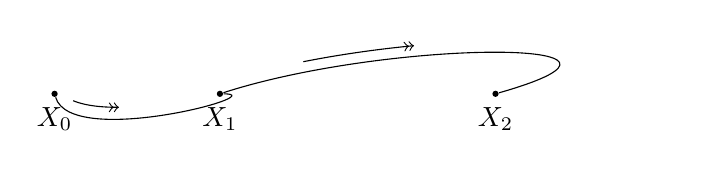
\begin{tikzpicture}[scale=0.70]

% First, define nodes
\draw (0,0) node[circle, inner sep=0.8pt, fill=black, label={below:{$X_0$}}] (E) {};  
\draw (3,0) node[circle, inner sep=0.8pt, fill=black, label={below:{$X_1$}}] (F) {}; 
\draw (8,0) node[circle, inner sep=0.8pt, fill=black, label={below:{$X_2$}}] (H) {};

% Draw the curved line. No to[bend] is allowed, only explicit control points
\draw  (E) .. controls +(0.3,-1) and +(1,0).. (F);
% Now, repeat the same curve, shifted up, and define 20 inner points named
% p1, p2, p3, etc.. for positions 0.15, 0.16, 0.17, etc up to 0.35 inside that curve
\path  ($(E)+(0,0.2)$) .. controls +(0.3,-1) and +(1,0) ..  ($(F)+(0, 0.2)$)
 {\foreach \t [count=\i] in {0.15,0.16,...,0.35} {  coordinate[pos=\t] (p\i) } };

% Finally draw the "curve" (polygonal line indeed) through those 20 inner points
\draw[->>] (p1) { \foreach \i in {1,...,20} {-- (p\i) } };

% Draw the curved line. No to[bend] is allowed, only explicit control points
\draw  (F) .. controls +(3.1,1) and +(3.5,1).. (H);
% Now, repeat the same curve, shifted up, and define 20 inner points named
% p1, p2, p3, etc.. for positions 0.15, 0.16, 0.17, etc up to 0.35 inside that curve
\path  ($(F)+(0,0.2)$) .. controls +(3.1,1) and +(3.5,1) ..  ($(H)+(0, 0.2)$)
 {\foreach \t [count=\i] in {0.15,0.16,...,0.35} {  coordinate[pos=\t] (p\i) } };

% Finally draw the "curve" (polygonal line indeed) through those 20 inner points
\draw[->>] (p1) { \foreach \i in {1,...,20} {-- (p\i) } };
\end{tikzpicture}
\caption{$f \ast f'$}
    \label{fig:my_label}
        
\end{center}

\end{figure}


\subsection{Fundamental Group}
Operation of $a \ast b$ might not always work. If $a$ and $b$ are in the same space, they cannot be jointed. We solve this issue by introducing fundamental group. 
\begin{mydef}\label{def:def444} 
 The easiest homotopy group: \\
        $$\pi_1(X,x_0)$$
\end{mydef}
Figure 5 shows the visual presentation of this group. It includes any path that starts at $X_0$ and ends at $X_0$.
\begin{figure}[hbt!]
\begin{center}

\begin{tikzpicture}[scale= 0.7]

% First, define nodes
\draw (0,0) node[circle, inner sep=0.8pt, fill=black, label={below:{$X_0$}}] (E) {};  
\draw (0,0) node[circle, inner sep=0.8pt, fill=black, label={below:{}}] (F) {}; 


% Draw the curved line. No to[bend] is allowed, only explicit control points
\draw  (E) .. controls +(4,2) and +(-1,3).. (F);
% Now, repeat the same curve, shifted up, and define 20 inner points named
% p1, p2, p3, etc.. for positions 0.15, 0.16, 0.17, etc up to 0.35 inside that curve
\path  ($(E)-(-0.3,0)$) .. controls +(4,2) and +(-1,3) ..  ($(F)-(-0.3, 0)$)
 {\foreach \t [count=\i] in {0.15,0.16,...,0.35} {  coordinate[pos=\t] (p\i) } };

% Finally draw the "curve" (polygonal line indeed) through those 20 inner points
\draw[->>] (p1) { \foreach \i in {1,...,20} {-- (p\i) } };

\end{tikzpicture}
\caption{Fundamental Group}
    \label{fig:my_label}
        
\end{center}
\end{figure}
\subsection{Fundamental Group of Surface}
Inspired from free group, surface can be generalized by the following polygonal scheme. 
\begin{mydef}\label{def:def444} 
Assign each edge with a label. Default direction is set as from $p_{k-1}$ to $p_{k}$.\\
Labelling scheme:
$$w = (a_1)^{\epsilon_1} \ast       (a_2)^{\epsilon_2} \ast    (a_3)^{\epsilon_3} \ast (a_4)^{\epsilon_4} \ast...        \ast(a_n)^{\epsilon_n} $$
where $\epsilon = \pm 1$  
\end{mydef}
Notice that this is just an element of the free group generated by the homoptopic equivalence class! Each $(a_i)^{\epsilon_i}$ is an element in the $G_\alpha$. A quick recap, $G_\alpha$ is an infinite cyclic group, so every n-fold of the $(a_i)$ is contained in this group. \\
The following two examples are a representation on what one can do using this scheme. 
\vspace{10mm}
 \begin{figure}[hbt!]
     \centering
     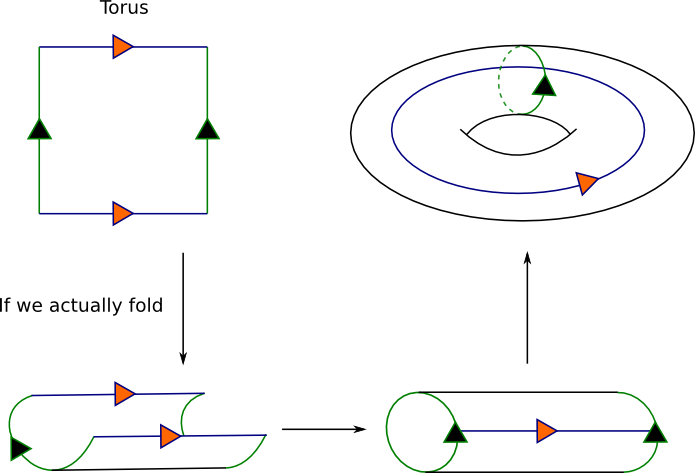
\includegraphics[scale=0.8]{2}
     \caption{torus}
     \label{fig:my_label}
 \end{figure}
$$w = a_1 \cdot b_{1}^{-1} \cdot a_{2}^{-1} \cdot b_2 \textbf{ and } a_1 \sim a_2, b_1 \sim b_2$$
 \begin{figure}[hbt!]
     \centering
     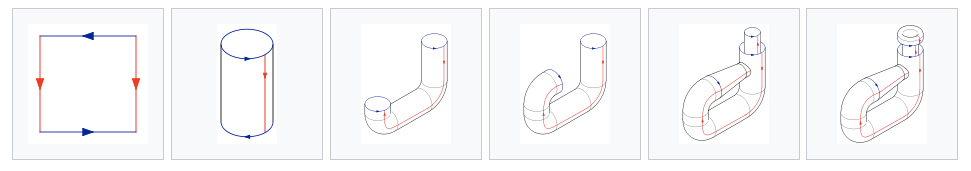
\includegraphics[scale=0.5]{3}
     \caption{Klein Bottle}
     \label{fig:my_label}
 \end{figure}
$$w = a_{1}^{-1} \cdot b_{1} \cdot a_{2}^{-1} \cdot b_2^{-1} \textbf{ and } a_1 \sim a_2, b_1 \sim b_2$$
Notice how much a difference it makes with different order. This is because it is not abelian. Fun fact: torus and klein bottle have a homomorphism relationship; they also have the same basis. 
\subsection{Homology by Group}
Torus has an interesting feature that can enable us to define homology from group: it is abelian and it might be most simple shape that is abelian.

\begin{mydef}\label{def:def444} 
The first dimension homology $H_1$ can be defined as:
$$H_1 = \pi_1[x_0,X] \hspace{1mm} / \hspace{1mm} [\pi_1[x_0,X],\pi_1[x_0,X]]$$
where $[G_1,G_2] = G_1G_2G_1^{-1}G_2^{-1}$, this is called commutator.
\end{mydef}
By doing the quotient,  $[G_1,G_2]$ is mapped to the identity element. So one can use $G_1G_2=G_2G_1$ relation in the $G$ group; therefore, now it is abelian. Commutator is often referred to as abelianizaiton function. 

\subsection{Homology by Vector Space}
It is much easier for one to comprehend the concept of homology in vector space. In vector space, quotient is called quotient vector space. The equivalent relation is simple minus operation.
\begin{mydef}\label{def:def444} 
$$H_n = ker(\partial_n) \hspace{1mm} / \hspace{1mm} Im(\partial_{n+1})$$
\end{mydef}
Kernel is the domain of  $\partial_n$ that maps to 0. In vector space, only cycle maps to 0. So $ker(\partial_n)$ is the group of every cycle. By quotienting the image $Im(\partial_{n+1})$ which is the boundary of the shape from the cycle, $H_n$ represents a connectivity between the n-dimensional shape and its boundary. The meaning of $H_n$ might be esoteric, in the next section, we will introduce a much more comprehensional concept: betti number. 
%%%%%%%%%%%%%%%%%%%%%%%%%%%%%%%%%%%%%%%%%%%%%%%%%%%%%%%%%%%%%%%%%%%%%%%%%%%%%%%%%%%%%%%%%%%%%%%%%%%%%%%%%%%%%%%%%%
\section{Dimension Problem}
\hspace{5mm} Now, as mentioned in the introduction, one of the most important applications in homology is Betti number. Betti number is simply the dimension of homology with the corrsponding dimension. By using a theorem in linear algebra, we can skip the tedious kernel and image formula and directly calculate the dimension of homology. This theorem is called rank-nullity theorem.
\subsection{Betti Number}
\large\textbf{Claim :} 
$$dim W + dim(V/W) = dim V$$
\newpage
\large\textbf{Proof :} 
\\[12pt]
\normalsize{
Firstly, we define the equivalent relation as $a \sim b$ if $a-b \in W $. In $V/W$,  $[a]+[b]=[a+b]$ define  (or $\overline{a} + \overline{b} = \overline{(a+b)}$ in some version) and $k \cdot [a] = [ka] $. Some useful properties of subspace $W$ are
$$W_i+W_j \in W|\forall i,j$$
$$c \cdot W \in W|c \in R$$
To show these two operations and the equivalent relation are valid,
\begin{indent} \begin{enumerate}
\item Equivalent relation has to satisfy all the properties of equivalence which are reflexivity, symmetry and transitivity. Let $v_i$ be any element in $V$. Since $W$ is a subspace, it contains $\{0\}$. Therefore, $v_i-v_i=0 \in W$. Based on the definition, $v_i \sim v_i$ for $\forall v_i \in V$. Let $v_i, v_j,v_m$ be three elements in $V$, if $v_i \sim v_j$, then $v_i-v_j=w_k \in W$. Since $v_j-v_i=-w_k \in W$, $v_j \sim v_i$. If $v_i \sim v_j$, $v_j \sim v_m$, then $v_i-v_j=w_k\in W$ and $v_j-v_m=w_o\in W$. $v_i-v_m=v_i-v_j+v_j-v_m=w_k+w_o \in W$, so $v_i \sim v_m$. Proven. (Exercise 3(a)i)
\item To define $\bigoplus$, let $\alpha \bigoplus \beta =\gamma$ and $\alpha_a \in \alpha$ and $\beta_a \in \beta$. In order to prove $\gamma=[\alpha_i + \beta_i]$ for $\forall i$, now we have to prove $[\alpha_a + \beta_a] = [\alpha_i + \beta_i] \Longleftrightarrow (\alpha_a + \beta_a) \sim (\alpha_i + \beta_i)$ based on the transitivity property. Since $\alpha_a$ and $\alpha_i$ are in the same equivalent group, $\alpha_a \sim \alpha_i$, which means $\alpha_a - \alpha_i=\alpha_a -\beta_a - (\alpha_i - \beta_a) \in W$. Similarly, $\beta_a \sim \beta_i$, which means $\beta_a - \beta_i=\beta_a -\alpha_a - (\beta_i - \alpha_a) \in W$. Since W is a subspace, $\beta_a -\alpha_a - (\beta_i - \alpha_a)+ \alpha_a -\beta_a- (\alpha_i - \beta_a)$ $= \alpha_a - \alpha_i+ \beta_a -\beta_i \in W$, so $(\alpha_a + \beta_a) \sim (\alpha_i + \beta_i)$ which is exactly what we are finding. Proven.
\item When defining $c \cdot v/w$, similar to defining $\bigoplus$, let $\beta:=c \cdot \alpha$ where $c \in R$. Let $\alpha_a$ be an element in $\alpha$,
so $c \cdot [\alpha_a]=[c \cdot \alpha_a]$. For $\forall i$, $\alpha_i-\alpha_a \in W$ since $\alpha_i \sim \alpha_a$. And $c \cdot \alpha_a -c \cdot \alpha_i \in W$ due to the properties of subspace mentioned before. Therefore, $(c \cdot \alpha_a) \sim (c \cdot \alpha_i) \longrightarrow \beta=[c \cdot \alpha_a] = [c \cdot \alpha_i]$. Proven.
\end{enumerate}
\end{indent}
\raggedleft\tiny{Source:Exercise 4a}
\\[15pt]
\raggedright
\normalsize{
Claim function Q as the $$Q : V \longmapsto V/W$$ $$a \longmapsto [a]$$

Lastly, by the rank - nullity theorem, which we will prove afterwards, 
$$rank(Q) + nullity(Q) = dim (V)$$
is equivalent to 
$$dim(Im(Q)) + dim(Ker(Q)) = dim (V)$$
For $ker(Q)$, it is the solution of $Q(x)=0$, which in another word, it is the set $ \{ x | x \sim 0 \} $. Claim: the $\{ x \}= W$ \\
(Exercise 3aii) proof: Let the equivalent class of $[0]$ be $\alpha$, our goal is to prove $\alpha=W \leftarrow \alpha \subset W,W \subset \alpha$. Let $\alpha_i$ be any element in $\alpha$. Since $\alpha_i \sim 0$, $\alpha_i-0=\alpha\in W$ for $\forall i$, so $\alpha \subset W$. On the other hand, for $\forall i$, since $W$ is a subspace of $V$, $\exists v_i=w_i=w_i-0$. Based on the definition of equivalent class, this $v_i$ will be categorized in the same equivalent class as $[0]$. Thus, for $\forall i$, $v_i \subset \alpha$ $\longrightarrow$  $w \subset \alpha$. Combine the two, we obtain $\alpha=w$. \\  So $nullity(Q)=dim(ker(Q))=dim (W)$. \\[5pt]
For $Im(Q)$, it is just all equivalent class under $v/w$, so $dim(Im(Q))=dim(v/w)$, combine the two, we get:
$$dim(W)+dim(V/W)=dim(V)$$
As mentioned, this proof uses the rank - nullity theorem, and we are going to prove it right now.
Using same claim of function Q as above, let the set $\{S_1,S_2....S_n\}$ be the basis of $ker(Q)$ and let the set $\{R\}:=\{T\backslash S\}$ where $\{T_1,T_2....T_m\}$ is the basis of $V$. Based on the Steinitz Exchange Lemma, $dim(R)=m-n$. So $\{R\} =\{R_1,R_2....R_(m-n)\}$ \\[5pt]
And now we can prove that $Q(\{R\})$ is a generator of $V/W$
$$Im(Q)=span(Q(T))=span(Q(\{R\}\cup\{S\}))=Span(Q(\{R\})\cup Q(\{S\}))$$
$$=Span(Q(\{R\})\cup {0}=Span(Q(\{R\}) $$
We can also show that $Q(\{R\})$ is linearly independent. If we claim it is linearly dependent,then based on the properties of linearly dependency,
$$\exists\{D_i\}\ne 0,\sum_{i=1}^{m-n}D_i \cdot R_i=0$$
But $$Q(\sum_{i=1}^{m-n}D_i \cdot R_i)=Q(0)=0$$
This makes $\sum_{i=1}^{m-n}D_i \cdot R_i \in ker(Q)$, since $T\in ker(Q) \ne R$, this contradiction proves that $Q(\{R\})$ is linearly independent. Combine with the generator proof, we know that $Q(\{R\})$ is a basis of $V/W$. So 
$$rank(Q)+nullity(Q)=dim(Im(Q))+dim(ker(Q))=dim(Q(\{R\}))$$
$$+dim(\{S\})=dim(\{R\})+dim(\{S\})=m-n+n=m=dim(V)$$
The transition from rank and nullity to image and kernel can be easily proven by$rank(Q)=dim(Col(Q))=dim(Col(V/W))=rank(V/W)$ and nullity is self-explanatory \\
Proven
}
}



%%%%%%%%%%%%%%%%%%%%%%%%%%%%%%%%%%%%%%%%%%%%%%%%%%%%%%%%%%%%%%%%%%%%%%%%%%%%%%%%%%%%%%%%%%%%%%%%%%%%%%%%%%%%%%%%%
\subsection{Code}
\hspace{5mm} Following is a code that applies the rank-nullity theorem that we just went through.
\begin{verbatim}
#                   Honours Research--Topology   
#                            Ziang Wang
#    Code is for find the dimension of homology of graph (R^2) 
                           (Betti Number)
                               Python

"""Use .txt file for input, enumerate simplices,every simplex 
occupy a line. 
                     Edge needs to be in order!!!
                Cannot have more than 10 vertix or edge

         e.g
            {1,2,3,4,5,6} for 1-dimensional and {12,23,45} for 
            2-dimensional 
    write:
                    ////    1
                            2
                            3
                            4
                            5
                            6
                            12
                            23
                            45                  ////

                     in the txt file
"""
#create an object for the graph 
class Graph: 
     def __init__(self, Input_data):
         self.Input_data = Input_data
         #seperate the simplex array in to Edge and Vertix subarray
         self.Edge_data = []
         self.Vertix_data = []
         for element in self.Input_data:
             if element < 10:
                 self.Vertix_data.append(element)       #array
             if element >= 10:
                 self.Edge_data.append(element)         #array
     #functions get the result
     def get_Edge_data(self):
         return self.Edge_data 
     def get_Vertix_data(self):
         return self.Vertix_data

  
#function to put graph into a matrix
def Rank_of_the_graph(Edge_array, Vertix_array):
     import numpy as np
     Matrix = np.zeros([len(Vertix_array),len(Edge_array)], dtype = int)
     i = 0
     for element in Edge_array:
         Matrix[int(element) % 10 -1][i] = 1     
# boundry operator: ones digit minus tens digit
         Matrix[int(element) //10 -1][i] = -1     
         i += 1
     return np.linalg.matrix_rank(Matrix)     # rank is for d1

#homology function 
"""     H0 = ker(d0) / Im(d1), dim(H0) = dim(d0)-rank(d1)  
"""
def get_the_dimension_of_H0(Vertix_array, rank):
     return len(Vertix_array) - rank

"""     H1 = ker(d1) / Im(d2), dim(H1) =
(number of Edge - rank(d1)) - 0
"""
def get_the_dimension_of_H1(Edge_array, rank):
     return len(Edge_array) - rank

#Read the file, possible improvement:
#analysis several files at the same time
txtfile_path = input("Input txt file path please:\n")
file = open(txtfile_path,"r")                          # an object
Input_value = []
for number in file:
    Input_value.append(int(number))                    #array
file.close()

#add multiple graphes if there are many files
Graph1 = Graph(Input_value)
rank1 = Rank_of_the_graph(Graph1.get_Edge_data(),
Graph1.get_Vertix_data())

#final output
print("dim of H0 is", get_the_dimension_of_H0
(Graph1.get_Vertix_data(), rank1))
print("dim of H1 is", get_the_dimension_of_H1
(Graph1.get_Edge_data(), rank1))
\end{verbatim}
%%%%%%%%%%%%%%%%%%%%%%%%%%%%%%%%%%%%%%%%%%%%%%%%%%%%%%%%%%%%%%%%%%%%%%%%%%%%%%%%%%%%%%%%%%%%%%%%%%%%%%%%%%%%%%%%%%
\section{Conclusion}
\hspace{5mm} In this paper, we went over some fundamental definitions in general topology, cubical set, homology and a dimensional theorem. In group topology, one can define homology formally and rationalize the meaning of Betti number. Of course, topology goes beyond what we have mentioned. Quotient mapping is more general. The quotient vector space is just a special case of quotient mapping. Graph which we did not mentioned, use vector space to bring geometric shape into algebra. On can also use fundamental group to achieve the same affect. Topology in general, provide us with a way of solving geometric questions more generally, as geometric method tends to be definite for each case.
%%%%%%%%%%%%%%%%%%%%%%%%%%%%%%%%%%%%%%%%%%%%%%%%%%%%%%%%%%%%%%%%%%%%%%%%%%%%%%%%%%%%%%%%%%%%%%%%%%%%%%%%%%%%%%%%%%
\section{Bibliography}
Kaczynski Mischaikow Mrozek (2004) Computational Homology, Springer New York, NY. Published: 01 December 2010 \\[20pt]
Topology (2nd Edition) James R. Munkres Prentice Hall, Incorporated, 2000 - Topology

\newpage
\end{normalsize}
\end{document}

